\documentclass[UTF8]{ctexart}
\usepackage{geometry}
\geometry{left=2.0cm,right=2.0cm,top=2.5cm,bottom=2.5cm}
\usepackage{amsmath}
\usepackage{cite}
\usepackage{amsthm}
\CTEXsetup[format={\large\bfseries\heiti\textbf}]{section}
\usepackage{subfigure}
\usepackage[graphicx]{realboxes}
\usepackage{caption}
\usepackage{float}

\title{不同图像识别技术的对比与探究}
\author{孟悦琦\quad 朱宸慷\quad 杨钧博\quad 李昌玟\quad 尹容乎}

\begin{document}
\maketitle

\section{背景介绍}
随着城市化进程的加速,车辆数量激增,交通管理难度加大。
为了改善城市交通状况,保障出行安全,开发自动车辆识别系统势在必行。
开发一个车辆识别系统可以提高交通管理效率、提升交通安全性。同时,车辆识别模块可以应用在诸多方面的问题上。 \par

有很多CV的方法可以进行车辆识别,这里主要可以分为传统方法和神经网络方法。
传统主要包括支持向量机、马尔可夫网络等。其特点是图像识别使用的模型相对简单、包含的参数数量有限。
同时,传统方法可能很依靠数据集的选取,在不同的数据集上可能有截然不同的表现。 \par

在CV领域,2010年出现了基于深度神经网络的模型。例如AlexNet,便是基于卷积神经网络的模型。
AlexNet具有高于传统CV方法的识别准确度\cite{AlexNet}。
之后又出现了ResNet\cite{ResNet}等方法,进一步提升其识别的准确度。
近些年,又出现了YOLO模型。
YOLO是一种划时代的单阶段目标检测算法。YOLO使用单次前馈网络即可完成检测,检测速度极快;
整图预测充分利用全局信息,检测精度高,因此被广泛使用\cite{YOLO}。
另外还有,Transformer模型,其是一种采用自注意力机制的深度学习模型,这一机制可以按输入数据各部分重要性的不同而分配不同的权重。
通过借鉴Transformer的设计思想,Google设计出ViT模型,也是一种识别准确度颇高的模型,且具有很强开创性的模型\cite{Vision_Transformers}。
在此基础上Facebook开发出LeViT模型,是其进一步分演进和发展\cite{LeViT} \par

本文将通过对比传统模型和神经网络模型,来比较分析不同模型的优劣,并分析其中的原理。

\section{数据集介绍}
现在有很多开源的数据集。考虑到本文要使用一些传统方法进行识别,我们选择的数据集不宜太大。
最终我们选择了kaggle上的Multilabel car and color dataset\footnote{可以在网站https://www.kaggle.com/datasets/julichitai/multilabel-small-car-and-color-dataset中获取。}作为数据集。
在数据集中,共包含三个品牌各三种颜色的车辆图片数据。数据集的部分图片如下:

\begin{figure}[H]
    \centering
\subfigure[matiz blue]{
    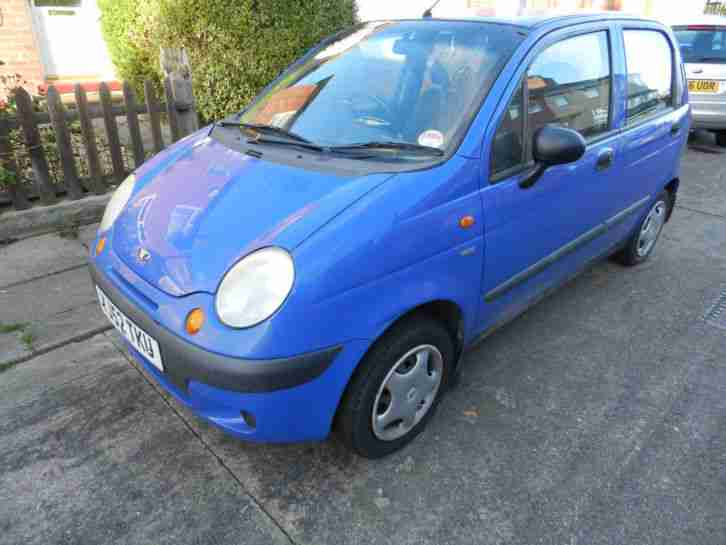
\includegraphics[width=3cm]{./dataset_graph/dataset_1.jpg}
    \label{matiz blue}
}\quad
\subfigure[tiggo black]{
    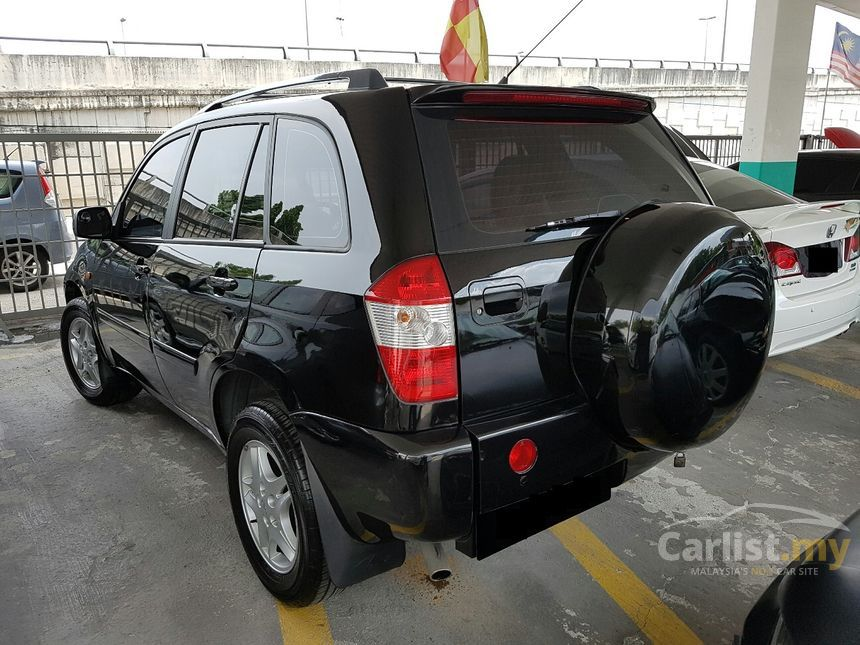
\includegraphics[width=3cm]{./dataset_graph/dataset_2.jpg}
        \label{tiggo black}
}\quad
\subfigure[rio blue]{
    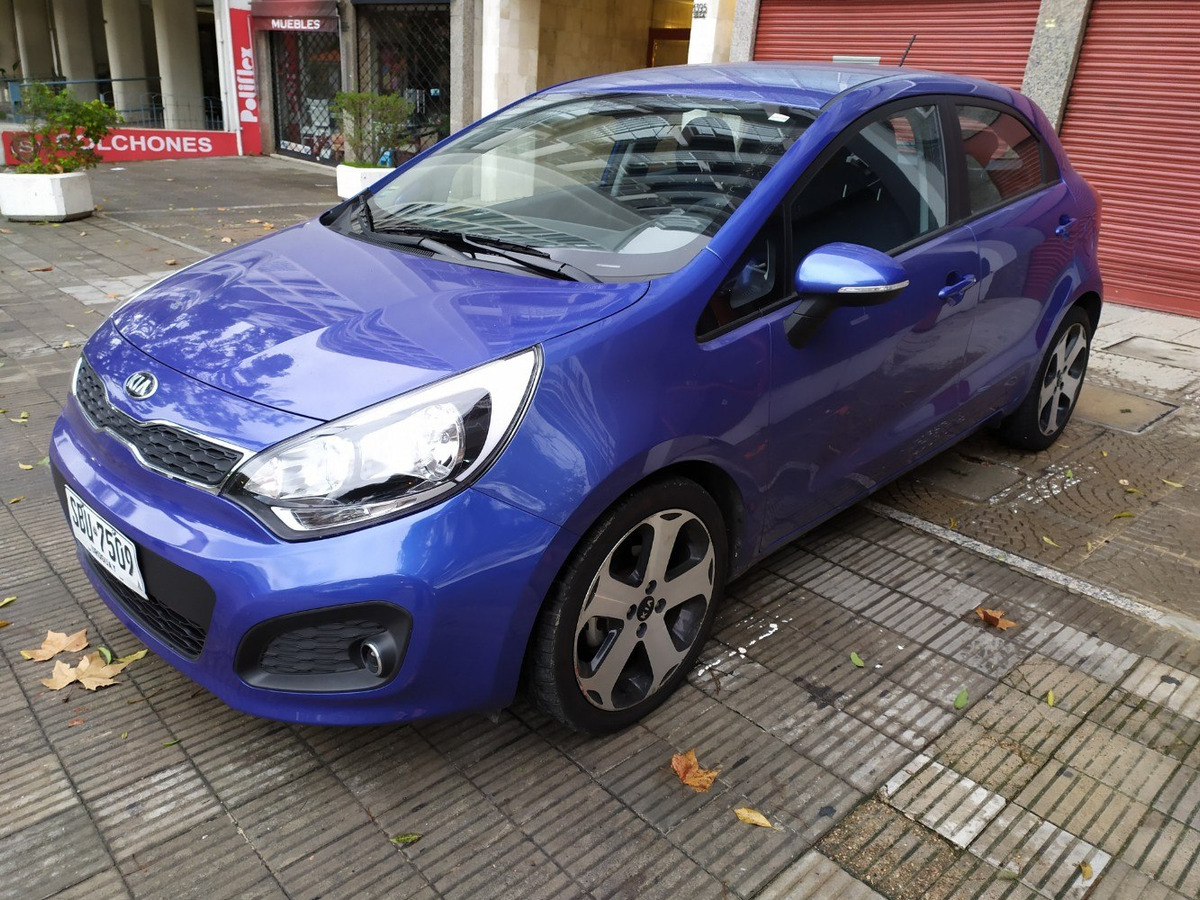
\includegraphics[width=3cm]{./dataset_graph/dataset_3.jpg}
    \label{rio blue}
}\quad
\subfigure[matiz red]{
    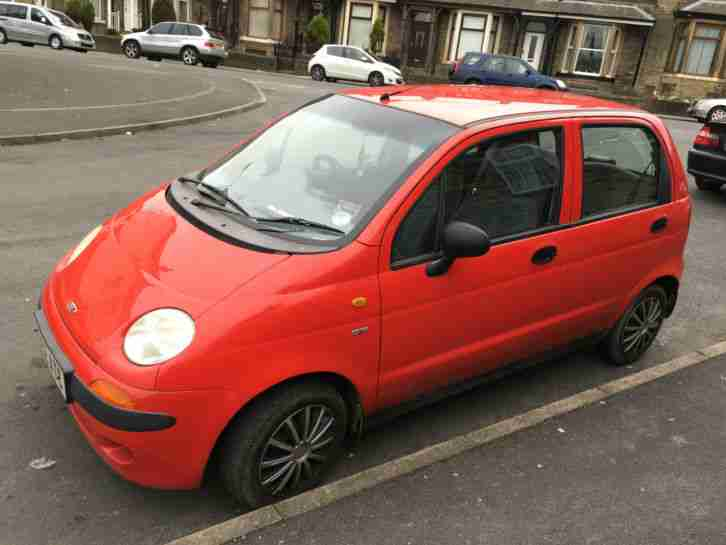
\includegraphics[width=3cm]{./dataset_graph/dataset_4.jpg}
    \label{matiz red}
}\quad
 
\caption{数据集样例}
\label{数据集样例}
\end{figure}

此数据集共有9个类,同时样本数量较少,不同品牌间视觉特征可能相近,如何提升模型泛化能力和防过拟合是关键。
此数据集很适合用来考察传统模型和神经网络之间的差别。

\section{AdaBoost对图像的识别分析}
\subsection{AdaBoost简介}

AdaBoost是Adaptive+Boosting的组合词,其算法的定义如下: \par
弱分类器(weak classifier)通过顺序(sequential)学习相互补充,并将它们组合在一起以最终提高强分类器(strong classifier)的性能。 \par

工作原理如下:\par
弱分类器(weak classifier)一次一个地顺序进行学习。首先学习的分类器会产生正确分类的数据和错误分类的数据。
首先学习的分类器将正确分类的结果信息和错误分类的结果信息传递给下一分类器。
下一分类器利用从前一个分类器接收到的信息来提高分类不佳的数据的权重(weight)。
也就是说,通过不断调整前一个分类器错误分类样本的权重,使其更集中于错误分类的数据,从而使学习效果更好。
因此,名称中带有“adaptive”。
最终分类器(strong classifier)通过对先前学习的弱分类器分别应用权重并进行组合来进行学习。 \par

总结一下,就是将预测性能较低的弱分类器组合在一起,最终形成一个性能稍好一些的强分类器。
弱分类器通过相互补充(adaptive)的方式进行学习,并通过组合这些弱分类器来形成一个分类器,因此称为 boosting。 \par

用公式表示如下:
\begin{gather}
    H(x) = \alpha_1 h_1(x) + \alpha_2 h_2(x) + \dots + \alpha_t h_t(x) = \sum_{t = 1}^{T} \alpha_t h_t(x)
\end{gather}
其中:\par
$H(x)$:最终强分类器,也称为加权多数投票分类器。 \par
$h$:弱分类器,也称为基分类器。 \par
$\alpha$:弱分类器的权重,用于衡量弱分类器对最终分类器的重要性。 \par
$t$:迭代次数,表示弱分类器的数量。 \par

\noindent AdaBoost 算法的工作原理如下: \par
1. 初始化训练数据集的每个样本的权重为 1/N,其中 N 是训练数据集的样本数。\par
2. 训练一个弱分类器。\par
3. 计算弱分类器的错误分类率。\par
4. 将错误分类率高的样本的权重增加,将错误分类率低的样本的权重减少。\par
5. 重复步骤 2-4,直到满足某个终止条件。\par
6. 将所有弱分类器的输出通过加权求和得到最终的强分类器的输出。\par


\noindent AdaBoost 算法具有以下优点:\par
1. 可以有效地提高弱分类器的性能。\par
2. 可以处理异常值。\par
3. 可以处理不平衡数据集。\par
4. AdaBoost 算法在分类、回归、异常检测等领域都有广泛应用。\par



\section{AlexNet对图像的识别分析}
\subsection{对AlexNet的介绍}
AlexNet 是一个深度卷积神经网络,它的结构如下:\cite{AlexNet}

\begin{figure}[H]
    \centering %表示居中
    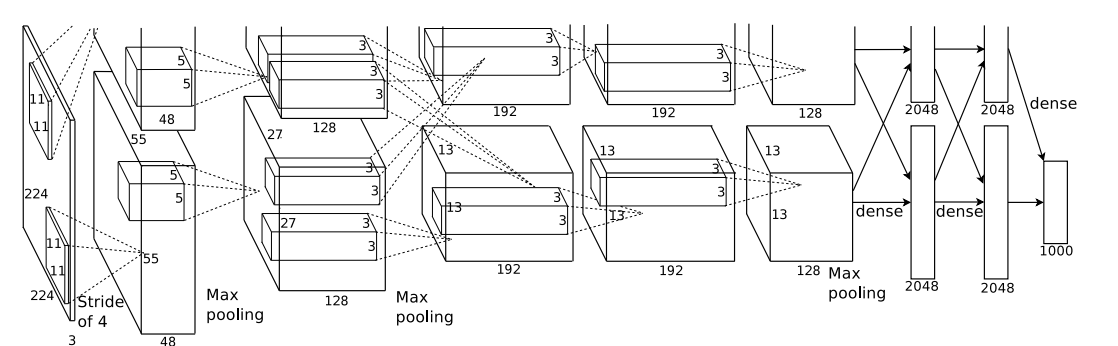
\includegraphics[height=4.5cm]{../AlexNet/AlexNet_arc.png}
    \caption{AlexNet结构}
\end{figure}

AlexNet 主要特点:\par
1. 更深的网络结构:AlexNet由 5 个卷积层、3 个全连接层和最后的 Softmax 分类层组成。 \par
2. ReLU 激活函数:AlexNet 是第一个大规模使用 ReLU 作为激活函数的网络,这加速了训练过程。 \par
3. Dropout:为了减少过拟合,AlexNet 在全连接层中使用了 Dropout。 \par
4. 局部响应归一化(LRN):在某些卷积层后使用了局部响应归一化。 \par
5. 数据增强:为了进一步减少过拟合,AlexNet 使用了图像平移、翻转和颜色变化等数据增强技术。 \par

\subsection{使用AlexNet对图像进行识别的效果分析}

训练结果如下:

\begin{figure}[H]
    \centering %表示居中
    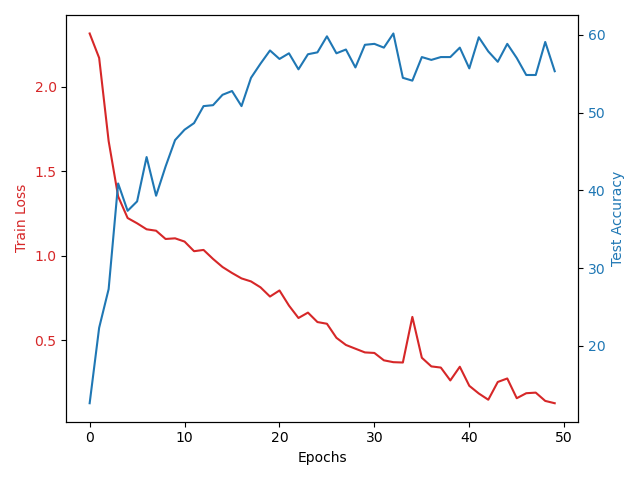
\includegraphics[height=4.5cm]{../AlexNet/AlexNet.png}
    \caption{AlexNet训练结果}
\end{figure}

在训练过程中,我们将数据集按 7:3 的比例划分为训练集和测试集。
采用 AlexNet 进行训练,训练 50 轮后,发现模型对于测试集的预测准确率不断上升,最后趋于稳定,稳定在 55\% 左右;
损失函数值也在不断下降,最终达到了 0.13。考虑到样本集中的数据量只有 2700 左右,数据量偏少,因此训练效果不是很理想。
如果增大样本集规模,模型预测的准确率应该会有进一步提升。 \par
在训练过程中发现,虽然损失函数值在下降,但是预测准确率却并未上升,有时甚至下降,这说明模型可能存在过拟合现象,这也可能是导致模型预测准确率不高的原因之一。

\newpage
\small
\bibliographystyle{IEEEtran}
\bibliography{ref}

\end{document}